% Préambule APMEP - Annales
% Auteurs
% tapuscrit : Jean-Paul Goualard
% relecture : François Kriegk et Denis Vergès
% figures TikZ : François Kriegk
% figures pstricks : Denis Vergès
% modifications :
% Remerciements :
% version 2 : 2026-07-12
\documentclass[12pt,a4paper,french]{article}
% Packages
%%% codage et police utilisée
\usepackage[T1]{fontenc}
\RequirePackage{iftex}
\iftutex % moteur utf-8 lualatex, xelatex
\usepackage{fourier-otf} % remplace fourier pour moteur utf8 (LuaLaTeX, XeLaTeX)
% Alternatives nécéssite (LuaLaTeX, XeLaTeX)
\usepackage{hyperref}
	%\usepackage{fontspec}% pour utiliser des fontes système
\else % pour les autres moteurs latex, pdflatex
\usepackage[utf8]{inputenc}
\usepackage{fourier}
\usepackage{amsmath,amssymb}
\usepackage[dvips]{hyperref}
\renewcommand{\ttdefault}{lmtt}
\fi
\usepackage[normalem]{ulem}
\usepackage{pifont}
\usepackage{lscape}
% tableaux
\usepackage{multicol}
\usepackage{multirow}
\usepackage{tabularx}
\usepackage{tabularray}
% texte et composition
\usepackage{textcomp}
\usepackage{babel}
\usepackage[np]{numprint}
%
\usepackage{fancyhdr}
\usepackage{makeidx}
\makeindex
% pour le symbole €
\usepackage{eurosym}
\DeclareRobustCommand{\officialeuro}{%
\ifmmode\expandafter\text\fi
{\fontencoding{U}\fontfamily{eurosym}\selectfont e}}
\AtBeginDocument{\renewcommand{\euro}{\officialeuro}}
% couleurs étendues
\usepackage{xcolor}
% pour les listes
\usepackage{enumitem}
% Enumérations réglage par défaut
\setlist[itemize]{label = \textbullet,leftmargin = 5mm,labelwidth = 3mm,labelsep = 2mm,align = left}
\setlist[enumerate]{labelindent = 0pt, leftmargin = 5mm, labelsep = 2mm, labelwidth = 3mm,labelsep = 2mm, align =  left}
\setlist[enumerate,1]{label  =  \textbf{\arabic*.}}
\setlist[enumerate,2]{label  =  \textbf{\alph*.}}
\setlist[enumerate,3]{label  =  \textbf{\roman*.}}
% pour l'ajustement des boites (figures…)
\usepackage{adjustbox}
% pour ne pas commencer un exercice en fin de page
\usepackage{needspace}
%
% Taille de la zone d'écriture
\usepackage[left = 1.5cm,right = 1.5cm,top = 3cm,bottom = 3cm]{geometry}
\setlength{\headheight}{15pt}
\setlength{\parindent}{0mm}
%
% Formatage du pdf
\hypersetup{%
pdfauthor  =  {APMEP},
pdfsubject  =  {Troisième, Série générale},
pdftitle  =  {Brevet des collèges    -- Session 2026},
allbordercolors  =  white,
pdfstartview = FitH
}
% Pour scratch (code)
\usepackage{scratch3}
% Pour le code Python
\usepackage{listings}
\lstdefinestyle{python}{
language = Python,
basicstyle = \ttfamily\small,
keywordstyle = \color{blue}\bfseries,
commentstyle = \color{gray}\itshape,
stringstyle = \color{orange},
numbers = left,
numberstyle = \tiny\color{gray},
breaklines = true,
frame = single,
backgroundcolor = \color{gray!5},
tabsize = 4
}
  % usage (exemple)
  %\begin{lstlisting}[style = python]
%def seuil():
%    n  =  1
%    p  =  0.5
%    while p < 0.6 :
%       n  =  n + 1
%       p  =  p*7/15 + 1/3
%    return n
%\end{lstlisting}
% Pour une visualisation de type tableur
\usepackage{pas-tableur}
%% pour PsTricks
\usepackage{pst-bezier}%% AVANT les autres PST
\usepackage{pstricks-add}
\usepackage{pst-func,pst-tree,pst-circ}
\usepackage{pst-eucl}
%% pour TikZ
\usepackage{tikz,pgfplots,pgf,tkz-tab,tikzpagenodes}
\usetikzlibrary{calc,patterns,decorations,arrows.meta,patterns.meta,arrows}
\pgfplotsset{compat = 1.18,/pgf/number format/.cd,use comma}
\usepackage{icomma} % gestion des espaces autour des virgules
\DeclareMathSymbol{;}{\mathbin}{operators}{"3B}% pour un espacement correct du ; en mode maths
%%%%%%%%%%%%%%%%%%%%%%%%%%%%%%%%%%%%%%%%%%
% Définitions
% notation en mode mathématique et hors mode mathématique
\newcommand{\R}{\ensuremath{\mathbb{R}}}
\newcommand{\N}{\ensuremath{\mathbb{N}}}
\newcommand{\D}{\ensuremath{\mathbb{D}}}
\newcommand{\Z}{\ensuremath{\mathbb{Z}}}
\newcommand{\Q}{\ensuremath{\mathbb{Q}}}
\newcommand{\C}{\ensuremath{\mathbb{C}}}
%
\providecommand{\up}{\textsuperscript}
%
\newcommand{\vect}[1]{\overrightarrow{\,\mathstrut#1\,}}
\newcommand{\vectt}[1]{\overrightarrow{\,\mathstrut\text{#1}\,}}
%
\def\Oij{$\left(\text{O};\vect{\imath},\vect{\jmath}\right)$}
\def\Oijk{$\left(\text{O};\vect{\imath},\vect{\jmath},\vect{k}\right)$}
\def\Ouv{$\left(\text{O};\vect{u},\vect{v}\right)$}
%
\newcommand{\ds}{\displaystyle}
%
\renewcommand{\d}{\mathrm{\,d}}
\renewcommand{\i}{\mathrm{\,i\,}}
\newcommand{\e}{\mathrm{\,e\,}}
%%%%%%%%%%%%%%%%%%%%%%%%%%%%%%%%%%%%%%%%%%%
\begin{document}
%---------------------------------------------------------
% Réglage entête, pied de page
%---------------------------------------------------------
\rhead{\textbf{A. P{}. M. E. P{}.}}
\lhead{\small Corrigé du brevet des collèges}
\lfoot{\small{Antilles, Guyane}}
\rfoot{\small{30 juin 2026}}
\pagestyle{fancy}
\thispagestyle{empty}
%---------------------------------------------------------
% Titre
%---------------------------------------------------------
\begin{center}\Large \bfseries
	\decofourleft~ Diplôme National du Brevet ~\decofourright\\[10pt]
	Série générale -- Antilles, Guyane -- 30 juin 2026
	\marginpar{\rotatebox{90}{\textbf{A. P{}. M. E. P{}.}}} \\[10pt]
	Corrigé
\end{center}

\section*{\centering PREMIÈRE PARTIE -- AUTOMATISMES}
\subsection*{Question 1}
Dans le repère, les coordonnées du point A sont A$(-2 ; 2)$.

\subsection*{Question 2}
Le point O est le milieu du segment [MK] donc le symétrique du point K par la symétrie centrale de centre O est M.

\subsection*{Question 3}
La formule pour calculer l'aire d'un triangle est \quad $\dfrac{\text{Base}\times \text{Hauteur}}{2}$.

Ici, en prenant [AC] comme base, la hauteur correspondante est [BD].

Le calcul attendu est donc :\quad $\mathrm{AC} \times \mathrm{BD}\div 2$.

Bonne réponse : \textbf{B.}

\subsection*{Question 4}
Les résultats obtenus sont : \emph{pile, pile, face, pile, face, face, face, face, pile, face}, soit 4 fois \emph{pile} sur 10 lancers.

La fréquence d'apparition de \og \emph{pile} \fg{} est :\quad  $\dfrac{\text{Nombre de \og{}\emph{pile}\fg{}}}{\text{Nombre de lancers}} = \dfrac{4}{10}$.

Bonne réponse : \textbf{C.}

\emph{Remarque} : la \og bonne \fg{} réponse est en fait $\dfrac25$.

\subsection*{Question 5}

On note $n$ un nombre entier.

%	Parmi les propositions suivantes, quelle expression donne la moitié de $n$ ?
La moitié de $n$ est $\dfrac{n}{2}$.

Bonne réponse : \textbf{D.}

\emph{Remarque :} $2n$ est le double de $n$, $n^2$ est son carré, et $n+2$ est la somme de $n$ et de 2.

\subsection*{Question 6}

1 h vaut 60 min, donc $\dfrac{1}{10}$ d'heure vaut $\dfrac{1}{10}\times 60 = \dfrac{60}{10}$, soit  $\np[min]{6}$.

Bonne réponse : \textbf{C.}

%	\begin{tblr}{*{4}{X}}
%		\textbf{A.}\quad 0,1 min &
%		\textbf{B.}\quad 1 min &
%		\textbf{C.}\quad 6 min &
%		\textbf{D.}\quad 10 min
%	\end{tblr}

\subsection*{Question 7}

La moyenne de cette série est $\dfrac{10+10+12+16}{4} = \dfrac{48}{4} = {12}$

\subsection*{Question 8}

La somme des mesures des angles d'un triangle est égale à $180$ en degré donc \quad
$x+x+120 = 180$ \quad d'où \quad $2x+120 = 180$,

ou en ajoutant $- 120$ à chaque membre :\quad $2x = 60$\quad donc\quad $x = 30$ (en degrés).

\subsection*{Question 9}

Si on note $v$ la vitesse moyenne, $d$, la distance parcourue et $t$ le temps de parcours, on a :

$v = \dfrac{d}{t}$ \quad donc \quad $vt = d$ puis $t = \dfrac{d}{v} = \dfrac{15}{20} = \dfrac{5\times 3}{5\times 4} = {\dfrac{3}{4}} = \dfrac{3 \times 15}{4 \times 15} = \dfrac{45}{60}$ en heure.
\quad
Le trajet dure  donc 45 min.

\needspace{15\baselineskip}
% saut de page si moins de 10 lignes disponibles
\section*{\hfill~ DEUXIÈME PARTIE (14 pts)\hfill~}

\section*{Exercice 1 (4 points)}

\begin{enumerate}
\item T, A et M sont alignés dans cet ordre donc

$\mathrm{TA} + \mathrm{AM} = \mathrm{TM}$ d'où $\mathrm{AM} = \mathrm{TM} - \mathrm{TA}$; or $7,7 - 2,2 = 5,5$ donc $\mathrm{AM} =  \np[m]{5,5}$.

\item Le triangle BAM est rectangle en A ; on lui applique le théorème de Pythagore.

$\mathrm{MB}^2 = \mathrm{AM}^2+\mathrm{AB}^2$ \quad donc\quad  $7,3^2  = \mathrm{AB}^2 + \mathrm{AM}^2 $ d'où AB$^2 = 7,3^2 - 5,5^2 = 53,29 - 20,25  = 23,04$.

$\mathrm{AB}>0$ \quad et \quad $\sqrt{23,04}=4,8$ \quad donc \quad  $\mathrm{AB} = \np[m]{4,8}$.

\emph{Remarque} : on pouvait voir que $a^2 - b^2 = (a + b)(a - b)$ et donc que
$7,3^2 - 5,5^2 = (7,3 + 5,5)(7,3 - 5,5) = 12,8 \times 1,8 = 6,4 \times 2 \times 3,6 = 64 \times \times 36 \times 0,01 = 8^2 \times 6^2 \times 0,1^2= (8 \times 6 \times 0,1)^2 = 4,8^2$ : on retrouve $\mathrm{AB} = \np[m]{4,8}$.

\item On sait que  dans le triangle BAM  rectangle en A on a par définition :

$\cos\left(\widehat{\text{ABM}}\right) = \dfrac{\text{longueur du côté adjacent}}{\text{longueur de l'hypoténuse}} = \dfrac{\text{AB}}{\text{MB}} = \dfrac{4,8}{7,3}  \approx \np{0,6575}$.

La calculatrice donne : $\widehat{\text{ABM}}\approx 48,9\degres$ soit environ 49\degres{} au degré près.

	\item \begin{itemize}
		\item E, A et B sont alignés dans cet ordre ;
		\item T, A et M sont alignés dans cet ordre ;
		\item $\dfrac{\mathrm{AE}}{\mathrm{AB}} = \dfrac{1,92}{4,8} = \dfrac{192}{480} = \dfrac{48}{120} = \dfrac{4}{10} = \dfrac25$ ; et $\dfrac{\mathrm{AT}}{\mathrm{AM}} = \dfrac{2,2}{5,5} = \dfrac{22}{55} = \dfrac25$.
	\end{itemize}

On a donc $\dfrac{\mathrm{AE}}{\mathrm{AB}} = \dfrac{\mathrm{AT}}{\mathrm{AM}}$ et d'après
 la réciproque du théorème de Thalès, les droites (TE) et (BM) sont parallèles.
	\item Si le triangle ABM est l'image du triangle AET par une homothétie de centre A, alors le côté homologue de [AT] (dans le triangle de départ) est [AM] (dans le triangle après l'homothétie). Le rapport de l'homothétie est donc $2,5$ ou $- 2,5$ car $\dfrac{\text{AM}}{\text{AT}} = \dfrac{5,5}{2,2} = \dfrac{55}{22} = \dfrac52 = 2,5$ et comme A (centre de l'homothétie est situé entre A et M le rapport est $- 2,5$.

Bonne réponse : \textbf{Proposition 3}.
\end{enumerate}

\needspace{10\baselineskip}
\section*{Exercice 2 (4 points)}

\begin{enumerate}
	\item On obtient successivement :
	\begin{itemize}
		\item $1- 2$ donc $-1$

		\item $(-1)\times 5$ donc $-5$

		\item $-5+3\times 1$ donc  $-5 + 3$ soit $-2$
	\end{itemize}
	Le résultat est $- 2$.

	\item On note $x$ le nombre choisi au départ.

	On obtient successivement :
	\begin{itemize}
		\item $x - 2$

		\item $5(x - 2)$ donc $5x - 10$

		\item $5x-10+3x$ donc $8x - 10$
	\end{itemize}

	Le résultat final est $8x-10$.

	\item
$\begin{array}[t]{@{} r r !{=} l}
\text{On résout l'équation: } & 8x-10 & 0\\
 \text{équivaut à: } & 8x & 10\\
 \text{équivaut à: } & x & \dfrac{10}{8}\\
 \text{équivaut à: } & x & 1,25
\end{array}$


	Pour que le résultat soit égal à 0, le nombre de départ doit être 1,25.

	\begin{enumerate}
		\item En partant de 1, on obtient successivement :
		\begin{itemize}
\item $4\times 1$ donc $4$
\item $4 - 5$ donc $-1$
\item $2\times (- 1)$ donc $-2$
		\end{itemize}

	Le résultat est $-2$.
		\item On applique le programme à un nombre $x$ quelconque.

	On obtient successivement :
\begin{itemize}
\item $4\times x$ donc $4x$
\item $4x-5$
\item $(4x-5)\times 2$ donc $8x - 10$
		\end{itemize}
On obtient donc le même résultat qu'avec le programme A.
	\end{enumerate}
\end{enumerate}

\needspace{10\baselineskip}
\section*{Exercice 3 (4 points)}

\begin{enumerate}
	\item Avec le tarif B, le prix payé pour douze demi-journées est, en euro : \quad $15 + 3,50\times 12 = 15 + 42 = 57$.
	\item \begin{itemize}
		\item  $f(x)$ représente le tarif payé pour $x$ demi-journées avec le tarif B : $f(x) = 3,5x + 15.$

Chaque demi-journée $x$ coûte en euro, $3,50$ donc un total de $3,5x$, auxquels on ajoute l'abonnement de 15\,\euro{}.

	\item $g(x)$ représente le tarif payé pour $x$ demi-journées avec le tarif C: $g(x) = 64$.

Le tarif est constant, égal à 64\,\euro{}, quel que soit le nombre de demi-journées..

	\item $h(x)$ représente le tarif payé pour $x$ demi-journées avec le tarif A: $h(x)=5,5x$.

Chaque demi-journée $x$ coûte en $5,50\,\euro$ donc un total de $(5,5x)$\,\euro{} pour $x$ demi-journées.
	\end{itemize}


	\item \begin{itemize}
		\item  $d_1$ est une droite dont l'ordonnée à l'origine est 15, donc est la représentation graphique de la fonction affine $f$.
		\item $d_2$ est parallèle à l'axe des abscisses, donc représente la fonction constante $g$.
		\item $d_3$ est une droite contenant l'origine ; elle représente la fonction linéaire $h$.
	\end{itemize}
	\item La droite ($d_1$) ne représente pas une situation de proportionnalité, puisque la fonction associée n'est pas linéaire. Graphiquement, la droite ne passe pas par l'origine du repère. $(f(0) \ne 0)$.
	\item On cherche à quel moment le tarif B, représenté par des points de la droite $(d_1)$ devient plus avantageux que le tarif A (représenté par des points de la droite $(d_3)$).

Plus avantageux, cela veut dire que cela coûte moins cher, pour le même nombre de demi-journées. On cherche donc à partir de quel antécédent les points de la droite $(d_1)$ sont  en-dessous des points de  la droite $(d_3)$.

C'est à partir de 8 demi-journées que le tarif B est plus avantageux.

\emph{Vérification} :

$\bullet~$ $f(7 ) = 3,5 \times 7 + 15 = 24,5 + 15 = 39,50$ et $h(7) = 5,5 \times 7 = 38,50$ , donc $f(7) > h(7)$ :

$\bullet~$ $f(8 ) = 3,5 \times 8 + 15 = 28 + 15 = 43$ et $h(8) = 5,5 \times 8 = 44$ , donc $f(8) < h(8)$.

	\begin{center}
		%Début Tikz
		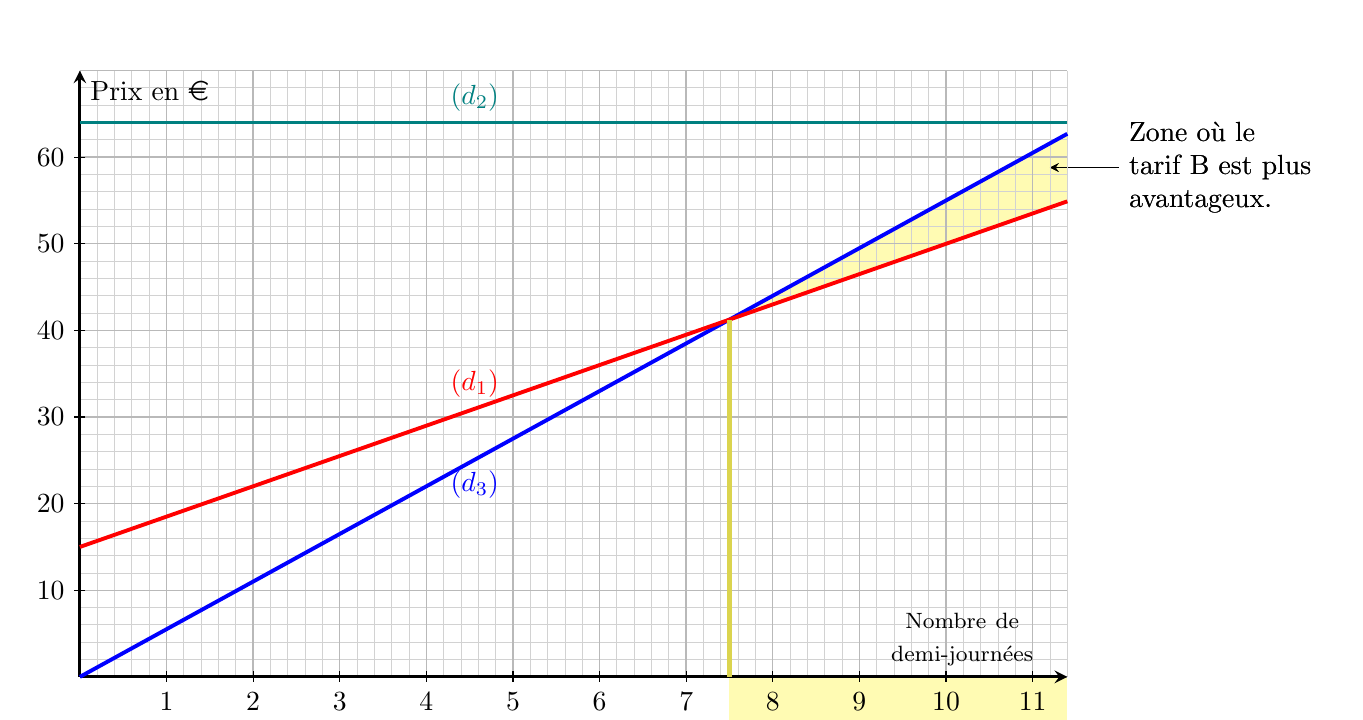
\begin{tikzpicture}[x = 11mm, y = 1.1mm, > = stealth]
			\fill[yellow!30] (7.5,41.25) --(11.4,62.7)--(11.4,54.9);
			\draw[<-] (11.2,58.8)--(12,58.8) node[right, text width=2.5cm]{Zone où le tarif B est plus avantageux.} ;
			\fill[yellow!30] (7.5,0) rectangle (11.4,-6.5);
			\draw[<-] (11.2,58.8)--(12,58.8) node[right, text width=2.5cm]{Zone où le tarif B est plus avantageux.} ;
			\draw[color  =  gray!35, line width  =  0.3pt, xstep = 0.2, ystep  =  2] (0,0) grid (11.4,70);
			\draw[color  =  gray!55, line width  =  0.5pt, xstep = 1, ystep  =  10] (0,0) grid (11.4,70);
			\draw[->,line width = 1pt] (0,0) -- (11.4,0) node[above left,text width = 2.4cm,align  =  center] {\footnotesize Nombre de demi-journées};
			\draw[->,line width = 1pt] (0,0) -- (0,70) node[below right] {Prix en \euro{}};
			\foreach \x in {1,...,11}
			\draw (\x,2pt) -- (\x,-2pt) node[below] {\np{\x}};
			\foreach \y in {10,20,...,60}
			\draw (2pt,\y) -- (-2pt,\y) node[left] {\np{\y}};
			\draw[teal,line width = 1.4pt] (0,64) -- (11.4,64) node[pos = 0.4,above]{$(d_2)$};
			\draw[blue,line width = 1.4pt] (0,0) -- (11.4,62.7) node[pos = 0.4,below]{$(d_3)$};
			\draw[red,line width = 1.4pt] (0,15) -- (11.4,54.9)
			node[pos = 0.4,above]{$(d_1)$};
			\draw[black!20!yellow!80, line width=2pt] (7.5,41.25)--(7.5,0) ;
		\end{tikzpicture}
		%Fin Tikz
		%		%Début PSTricks
		%		\psset{xunit = 1cm,yunit = 0.1cm,arrowsize = 2pt 3}
		%		\begin{pspicture}(-0.6,-5)(11,85)
			%			\psaxes[linewidth = 1.25pt,Dy = 10,labelFontSize = \scriptstyle]{->}(0,0)(0,0)(11,85)
			%			\multido{\n = 0+1}{12}{\psline[linewidth = 0.15pt](\n,0)(\n,85)}
			%			\multido{\n = 0+10}{9}{\psline[linewidth = 0.15pt](0,\n)(11,\n)}
			%			\psplot[plotpoints = 2000,linewidth = 1.25pt,linecolor = red]{0}{11}{3.5 x mul 15 add}
			%			\psplot[plotpoints = 2000,linewidth = 1.25pt,linecolor = blue]{0}{11}{5.5 x mul}
			%			\psline[linewidth = 1.25pt,linecolor = green](0,64)(11,64)
			%			\uput[u](9,0){\footnotesize Nombre de demi-journées}
			%			\uput[r](0,83){\footnotesize Prix en \euro}
			%			\rput(3,14){\blue $(d_3)$}\rput(3,30){\red $(d_1)$}\rput(3,66){\green $(d_2)$}
			%		\end{pspicture}
		%Fin PSTricks
	\end{center}

	\item \begin{enumerate}
		\item On veut traduire la fonction $f$ pour le tableur. \quad $f(x) = 15 + 3,5x$

		On peut procéder par élimination :
		\begin{itemize}
			\item \textsf{= 15+3,5*$x$}\quad ne convient pas, car le tableur ne connait pas $x$, il faut lui expliquer dans quelle cellule il trouvera la valeur $x$ correspondant à ce que l'on veut afficher;
			\item \textsf{= 15+3,5*1}\quad ne convient pas. Le résultat affiché dans la cellule \textsf{B3} serait correct, \textbf{mais}, on veut que la formule soit correcte \emph{étirée vers la droite}. Si on étire cette formule vers la droite, le calcul sera toujours le même, le 1 ne sera pas remplacé par 2, 3 et ainsi de suite;
			\item \textsf{= 15+3,5*B1}\quad est donc la bonne formule, par élimination, et parce que c'est bien dans la cellule \textsf{B1} que l'on va trouver l'antécédent du tarif que l'on veut calculer.
		\end{itemize}

		La formule à taper est donc :\quad\textsf{  = 15+3,5*B1.}

		\item Le tarif C devient plus avantageux à partir de la 14\up{e} demi-journée, le prix devenant supérieur ou égal à 64. (la cellule \textsf{P2} contient un nombre plus grand que 64).

Le tableur indique $64,5$ mais le résultat en euro et cent d'euro est $64,50$.

		\emph{Vérification par le calcul (non demandée) :}

$3,5x + 15 <  64$ \quad revient à \quad $3,5x<  64-15
	$ ou $3,5x <  49$ \quad donc \quad $x < \dfrac{49}{3,5}$.

Comme \quad $\dfrac{49}{3,5} = \dfrac{490}{35} = \dfrac{7\times 70}{7\times 5} = \dfrac{70}{5} = 14$, \quad on retrouve bien le résultat : à partir de 14 demi-journées.
	\end{enumerate}
\end{enumerate}
\end{document}
